%!TEX root = ../thesis.tex
\chapter{Generalized static mass distribution with the LTB metric}
\label{appendix:ltb}

In this section we generalize the model from a point mass vacuole to a vacuole with an arbitrary static mass distribution. In order to do that, the Kottler metric has to be replaced with another metric. 

We use the Lema\^itre-Tolman-Bondi (LTB) model \citep{tolman1934effect,bondi1947spherically,lemaitre1933expansion}, which is the most general spherically symmetric solution of Einstein`s field equations without the assumption of spatial homogeneity. It has FRW model as a special sub-case. The model was originally a dust model but was later extended to include pressure \citep{lasky2006generalized}, and this pressure term is needed to achieve a static system. The metric is given by

\begin{equation}
  ds^2 = A(R)^2 dT^2 - \frac{dR^2}{f(R)} - R^2 d \Omega^2.
  \label{eq:ltb-metric}
\end{equation}
where $f(R)$ is given by \autoref{eq:kottler-metric-f}. This is very similar to the Kottler metric except that the mass term in $f(R)$ is now a function of radius and there is an new term $A(R)$. Solving the EFEs for this metric yield the usual Tolman-Oppenheimer-Volkoff (TOV) equations \citep{tolman1939static,oppenheimer1939massive} for a static stellar interior, which give us the variation of $A(R)$ with $R$ as

\begin{equation}
  A_{,R} = - A \frac{P_{,R}}{\rho + P}
  \label{eq:alpha-evolution}
\end{equation}
where $P$ changes with $R$ as

\begin{equation}
  P_{,R} = \frac{\rho + P}{2\left (1- \frac{2M}{R} - \frac{\Lambda R^2}{3}\right )R}
  \left (\frac{2 \Lambda R^2}{3}  -3PR^2 -\frac{2M}{R} \right ) 
  \label{eq:pressure-P-evolution}
\end{equation}
and $M$, $\rho$ are quantities that depend on $R$. 


On the matching surface, the metric reduces to the Kottler metric. Therefore the boundary conditions given in \autoref{chapter:swiss-cheese} remains valid. In addition, there are boundary conditions on $P$ and $A$, given by

\begin{equation}
  P = 0
\end{equation}

\begin{equation}
  A^2 = \sqrt{1- \frac{2M}{R} - \frac{\Lambda R^2}{3}}.
\end{equation}

The null geodesic equations expressed in terms of these quantities are

\begin{subequations}
  \begin{align}
    \dot{T} &= \frac{E}{A(R)^2}\\
    \ddot{R} &= \frac{E^2}{2}\left ( \frac{f_{,R}}{\alpha^2} - \frac{2f\alpha_{,R}}{\alpha^3} \right ) - \frac{L^2}{2} \left ( \frac{f_{,R}}{R^2} - \frac{2f}{R^3} \right )\\
    \dot{\phi} &= \frac{L}{R^2}
  \end{align}
  \label{eq:ltb-null-geodesics}
\end{subequations}
where $E = A^2\dot{T}$ and $L = R^2\dot{\phi}$ are constants of the motion, and $f_{,R}$ is given by

\begin{equation}
  f_{,R} = \frac{2M}{R^2} - 8\pi \rho R - \frac{2 \Lambda R}{3}.
\end{equation}

These equations combined with \autoref{eq:alpha-evolution} and \autoref{eq:pressure-P-evolution} determine the trajectory of light through this metric. 

We use the NFW profile \citep{navarro1996structure} for the mass distribution to model a physically motivated galaxy. In this profile the density is

\begin{equation}
  \rho(R) = \frac{\rho_0}{\frac{R}{R_s} \left ( 1 + \frac{R}{R_s} \right )^2}
  \label{eq:nfw-density}
\end{equation}
where $R_s$ is the scale radius. Given a radius $R_{\text{max}}$, the total mass is given by

\begin{equation}
  M_{\text{total}} = 4\pi \rho_0 \left [  \ln \left ( \frac{R_s + R_{\text{max}}}{R_s} \right ) - \frac{R_{\text{max}}}{R_s + R_{\text{max}}} \right ]
  \label{eq:nfw-total-mass}
\end{equation}
and since total mass is fixed then we can find $\rho_0$. $R_s$ can also be expressed in terms of the virial radius $R_{\text{vir}}$ and the halo concentration parameter $c$

\begin{equation}
  R_s = \frac{R_{\text{vir}}}{c}.
\end{equation}

If we assume that the extent of the mass distribution is very small compared to the distances between the source, lens, and observer, then this justifies the thin-screen approximation, which states that the mass distribution of the lens can be treated as if it were an infinitely thin mass sheet perpendicular to the line-of-sight. Since we have a spherically symmetric mass distribution, the lensing mass is given by
\begin{equation}
  M(R_u) = 2\pi \int_0^{R_u} \Sigma(R) R dR
  \label{eq:ltb-projected-mass}
\end{equation}
where $R_u$ is as defined in \autoref{chapter:swiss-cheese} and $\Sigma(R)$ is the projected surface density
\begin{equation}
  \Sigma(R) = \int \rho(R, z) dz 
  \label{eq:ltb-projected-surface-density}
\end{equation}
where $z$ is in the direction connecting the lens, observer, and source. \autoref{eq:ltb-projected-mass} represents the mass contained within a cylinder of radius $R_u$, with an axis parallel to the ray and passing through the centre of the lens. 

Substituting in the density for a NFW mass profile, the lensing mass $M_p$ for a given $R_u$ is given by (Eq. 43 of \citet{lokas2001properties})

\begin{equation}
  M_p(R) = \frac{M_{\text{total}}}{\ln\left ( \frac{R_s + R_{\text{max}}}{R_s}\right) - \frac{R_{\text{max}}}{R_s + R_{\text{max}}}} \left [\frac{C^{-1}(R_{\text{vir}}/R)}{\mathopen| R^2/R_{\text{vir}}^2 - 1 \mathclose|^{1/2}} + \ln \left ( \frac{R}{2 R_{\text{vir}}}\right ) \right ]
\end{equation}
where $C^{-1}$ is the function
\begin{equation}
  C^{-1}(x) = 
  \begin{cases}
    \cos^{-1}(x)  & R > R_s\\
    \cosh^{-1}(x) & R < R_s
  \end{cases}
\end{equation}
If the light ray does not pass through the mass at all, or if we supply a point mass for the mass distribution, then the result reduces to that of a Kottler Swiss-Cheese. This was used to check the robustness of the code. 

\begin{figure}
\centering
\subcaptionbox[Short Subcaption]{%
    Density%
}
[%
    0.5\textwidth % width of caption
]%
{%
    \includegraphics[width=0.5\textwidth]%
    {images/ltb-density.png}%
}%
% \hspace{0.1\textwidth} % seperation
\subcaptionbox[Short Subcaption]{%
    Mass%
}
[%
    0.5\textwidth % width of caption
]%
{%
    \includegraphics[width=0.5\textwidth]%
    {images/ltb-mass.png}%
}%

\subcaptionbox[Short Subcaption]{%
    Pressure%
}
[%
    0.8\textwidth % width of caption
]%
{%
    \includegraphics[width=0.5\textwidth]%
    {images/ltb-pressure.png}%
}%
\caption[Short Caption]{Plot of the mass, density, and pressure functions for $\Omega_{\Lambda} = 0$. The radial coordinate is expressed in terms of $R_{h0} = r_h$, the initial size of the Kottler hole. The density and pressure are expressed in terms of the density of the initial FRW density $\rho_m$. Density is truncated at $R = r_h/2$. We use $c = 10$ and $R_{\text{vir}} = r_h/100$}.
\label{fig:ltb-quantities}
\end{figure}

We use $c = 10$ which roughly corresponds to the masses of bright galaxies \citep{lokas2001properties}. Density was truncated at $R_{\text{max}} = r_h/2$ to take into account the volume change of the hole in static coordinates as the universe expands. We set $R_{\text{vir}} = r_h/100$. For these parameters, the density, mass, and pressure functions are plotted in \autoref{fig:ltb-quantities}. 

\autoref{fig:ltb-results} shows the results of the numerical simulations in flat space when compared with the conventional, Rindler \& Ishak, and Kantowski's predictions. 

\begin{figure}
  \centering
  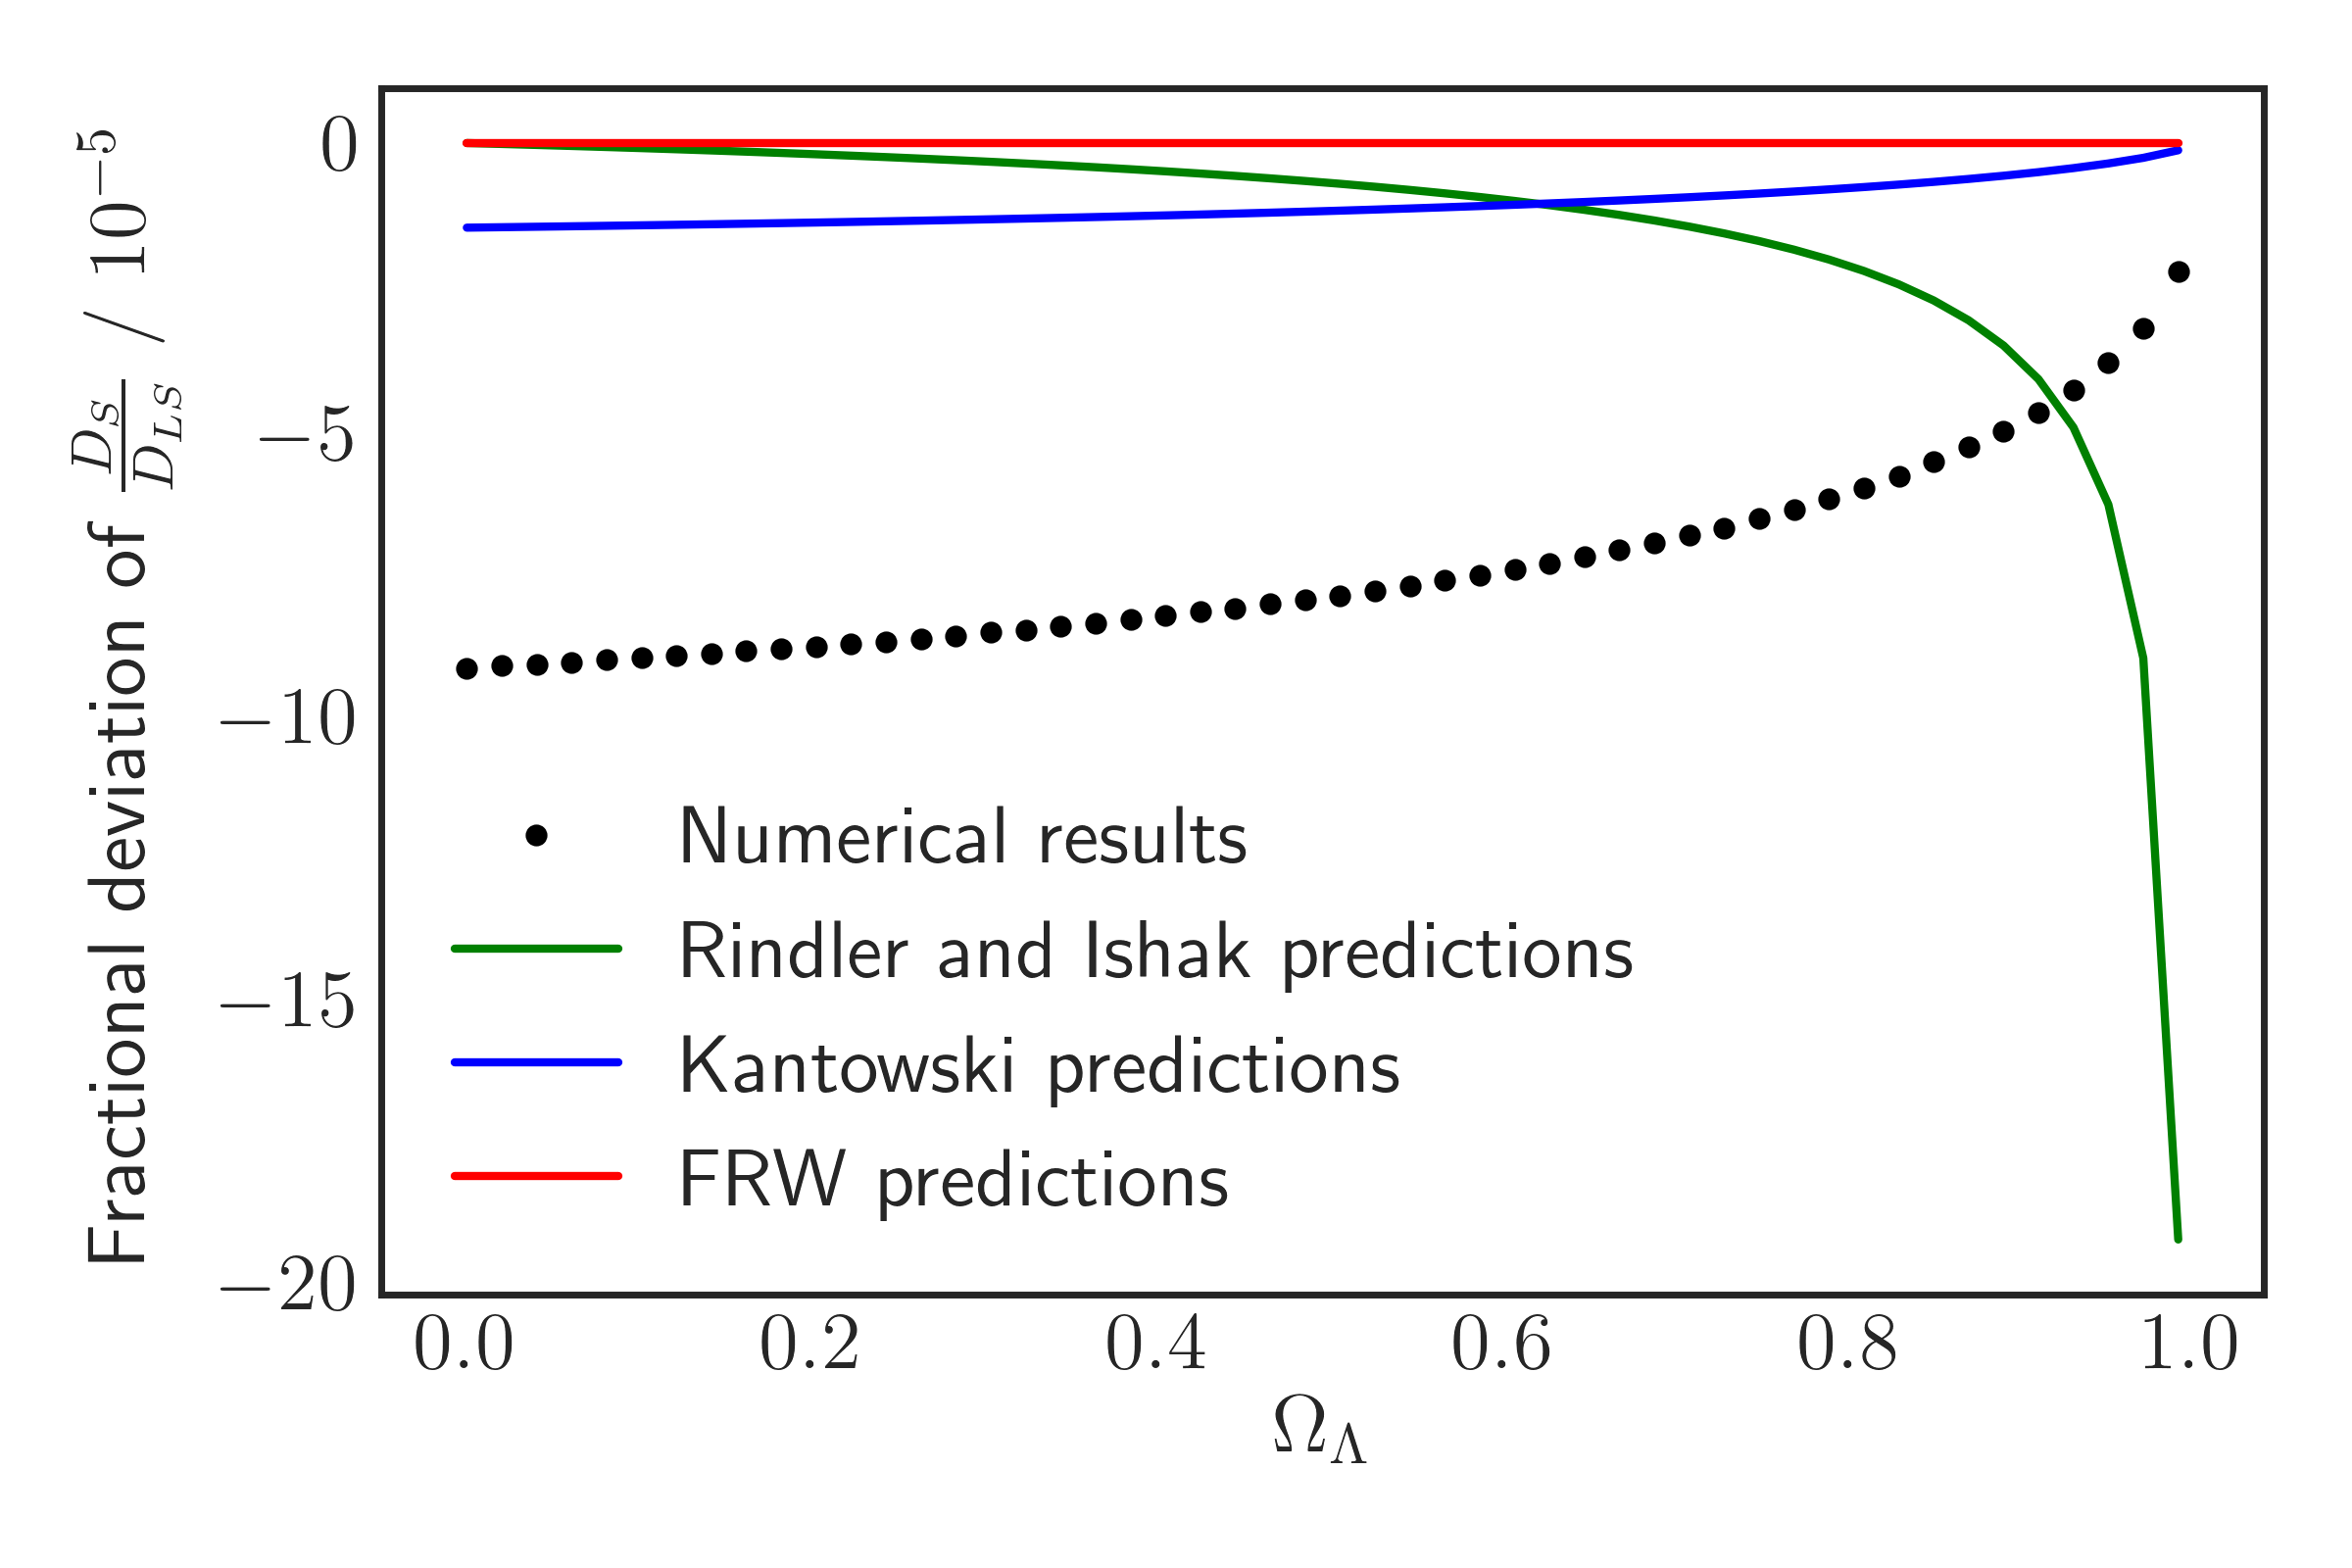
\includegraphics[height=0.5\linewidth]{images/ltb.png}
  \caption{Results for the LTB model with parameters $c = 10$, $M_{\text{total}} = 10^{12} M_\odot$, $\theta_E = 0.5^{\prime\prime}$, $R_{\text{max}} = r_h/2$, $R_{\text{vir}} = r_h/100$. Numerical results are plotted as a fractional deviation from the conventional FRW lensing predictions, as are the Rindler \& Ishak and Kantowski predictions. }
  \label{fig:ltb-results}
\end{figure}

The results show the same general trend as the Kottler case, except now the there is a bigger discrepancy between the conventional result and the numerical result. This is likely the error induced by the thin-screen approximation. \citet{frittelli2011accuracy} found that the thin lens approximation when applied to the NFW mass profile produced an error of similar magnitude. 